\documentclass[11pt,a4paper]{ctexart}
\usepackage[margin=2.15cm]{geometry}
\usepackage{amsmath,amssymb,bm,booktabs,array,longtable,graphicx,xcolor,hyperref,siunitx,float}
\hypersetup{colorlinks=true,linkcolor=blue!55!black,urlcolor=blue!55!black}
\graphicspath{{../results/}{../results/absolute/}{../results/residual/}}
\title{EXP-018：局部耦合扰动下的逐匝异构 GNN 实验报告}
\author{高频变压器智能建模实验线}
\date{2026年9月10日}

\begin{document}
\maketitle
\begin{abstract}
本实验回答一个受控但关键的问题：当高频变压器的局部电容、跨绕组电容和局部磁耦合发生变化时，显式区分物理边类型的逐匝异构图网络，是否比将全部耦合压成同一邻接关系的 FALCON 风格同质图网络更有优势。实验以 EXP-015 精确矩阵/Kron 求解器为物理教师，构造 $4+4$、$6+6$ 和 $8+8$ 三种逐匝图，在 DAB 自然 PWM 奇次谐波条件下预测端口导纳、内部节点电压和跨绕组位移电流。结果表明：直接学习绝对响应时，异构模型没有超过同质基线；改为学习相对同工况标称模型的局部残差后，edge-centric 异构模型相对 FALCON 在端口响应和内部电压 MAE 上分别改善 $4.84\%$ 和 $5.58\%$，但跨绕组边电流误差反而恶化约 $1.65\%$，局部峰值定位也仍较弱。因此，本实验只证明了关系类型在“局部扰动传播”任务上存在有限价值，尚未证明异构 GNN 对所有局部任务全面占优。
\end{abstract}

\section{实验目的与研究边界}
前一阶段 EXP-016 已打通图数据、CUDA 训练和精确物理教师链路，但其八个扰动参数主要是全局尺度，边类型并未真正承担局部信息。EXP-018 将扰动下沉到匝级和边级，并把内部响应加入监督，从而检验异构边设计是否有必要。

本实验是算法预实验，\textbf{不是} COMSOL、Simulink 开关器件全模型或实物结论。DAB 仅由自然 PWM 奇次谐波及其工况条件表示；负载量使用由 DAB 基本关系计算的代理量，不是独立负载动态；未包含死区、器件 $C_{\mathrm{oss}}$、探头链路、接地阻抗和温度漂移。

\section{物理教师与数学模型}
\subsection{逐匝网络方程}
将原副边每个匝段视为一个节点。串联支路构成阻抗矩阵
\begin{equation}
 \bm Z_s(\omega)=\bm R+j\omega\bm L,
\end{equation}
其中 $\bm L$ 保留全局主磁通的低秩耦合和局部漏磁耦合。节点电容矩阵 $\bm C$ 由纵向电容、对地电容及非局部跨绕组 $C_{ps,ij}$ 盖章得到。若 $\bm A$ 是支路-节点关联矩阵，则节点导纳为
\begin{equation}
 \bm Y_n(\omega)=\bm A^{\mathsf T}\bm Z_s^{-1}(\omega)\bm A+j\omega\bm C.
\end{equation}
将端口节点记为 $p$、内部节点记为 $i$，分块后采用 Kron 消元：
\begin{equation}
 \bm Y_{port}=\bm Y_{pp}-\bm Y_{pi}\bm Y_{ii}^{-1}\bm Y_{ip}.
\end{equation}
在给定端口电压 $\bm v_p$ 时，内部电压为
\begin{equation}
 \bm v_i=-\bm Y_{ii}^{-1}\bm Y_{ip}\bm v_p.
\end{equation}
跨绕组电容边 $(i,j)$ 的第 $k$ 次谐波位移电流为
\begin{equation}
 I_{ps,ij,k}=j\omega_k C_{ps,ij}\left(V_{p,i,k}-V_{s,j,k}\right),
\end{equation}
多谐波 RMS 标签由 $\sqrt{\sum_k |I_{ps,ij,k}|^2}$ 构造。

\subsection{DAB 自然谐波条件}
使用 $m\in\{1,3,5,7,9\}$ 的奇次谐波，$\omega_m=2\pi m f_s$。训练/验证相移范围为 $5^\circ$--$35^\circ$，测试扩展到 $35^\circ$--$50^\circ$；电压比训练/验证为 $0.9$--$1.1$，测试扩展到 $0.8$--$0.9$ 或 $1.1$--$1.2$。有限边沿时间通过高频衰减因子进入谐波幅值。这一划分专门检验跨工况泛化，而非随机同分布拆分。

\section{局部扰动与图数据契约}
每个样本从同拓扑标称模型出发，独立施加局部 $R_i$、漏感、平滑纵向/对地电容扰动；跨绕组电容使用带状稠密 $C_{ps,ij}$ 并叠加局部面对区域 patch；磁耦合由主磁通低秩项和局部低秩漏磁项共同构造。这样避免 EXP-016 中“只随机八个全局尺度”的问题。

节点特征包含绕组编号、归一化位置、端口标志、局部 $R_{ii}/L_{ii}$ 以及 DAB 工况。边被分成四类：串联导电边、局部电容边、跨绕组电容边、全局/非局部磁耦合边。图级标签为五个谐波上的 $Y_{11},Y_{22},Y_{12}$ 幅相；节点标签为内部复电压；边标签为每条 $C_{ps,ij}$ 的位移电流对数值。

\section{对照网络与损失函数}
\begin{enumerate}
 \item \texttt{falcon\_homogeneous}：全部物理关系合并为同质加权消息传递；
 \item \texttt{hft\_typed}：四类关系独立聚合，但每类只使用标量边权；
 \item \texttt{edge\_centric\_hetero}：每类独立 edge MLP，显式融合发送节点、接收节点、边值、距离和工况，并设置跨绕组边读出头。
\end{enumerate}
三者接受相同输入、相同监督和相同数据划分。联合损失为
\begin{equation}
 \mathcal L=\lambda_g\mathcal L_Y+\lambda_n\mathcal L_V+\lambda_e\mathcal L_{I_{ps}}.
\end{equation}

实验包含两种目标：绝对目标直接预测物理响应；残差目标预测同一拓扑、同一 DAB 工况下，相对标称图的变化
\begin{equation}
 \Delta\bm y=\bm y(\mathcal G,\bm c)-\bm y(\mathcal G_0,\bm c).
\end{equation}
残差设计不是人为“让异构网络变好”，而是消除共同工况造成的大幅全局分量，使任务真正关注局部图变化。

\section{可复现设置与物理合规检查}
随机种子为 1809，训练/验证/测试样本数为 720/150/240，训练 55 个 epoch，设备为 NVIDIA GeForce RTX 5070 CUDA。物理教师检查结果如下：
\begin{center}
\begin{tabular}{lr}
\toprule
检查项 & 数值\\
\midrule
最大互易性误差 & $1.32\times10^{-14}$\\
最小实部导纳特征值 & $3.31\times10^{-7}$\\
最大内部 KCL 残差 & $5.11\times10^{-11}$\\
\bottomrule
\end{tabular}
\end{center}
上述结果说明教师网络满足数值互易性、测试样本中的无源性和内部节点平衡，但不证明参数对应某一真实样机。

\section{结果}
\subsection{绝对响应学习}
\begin{center}
\begin{tabular}{lrrrr}
\toprule
模型 & 端口 MAE & 节点 MAE & 边电流 log-MAE & 参数量\\
\midrule
FALCON 同质图 & \textbf{0.03459} & 0.02173 & \textbf{0.07419} & 57,449\\
HFT typed & 0.04137 & \textbf{0.02139} & 0.09781 & 86,177\\
Edge-centric hetero & 0.03685 & 0.02255 & 0.08635 & 164,129\\
\bottomrule
\end{tabular}
\end{center}
绝对任务中，异构模型没有形成总体优势。FALCON 在端口和边电流上最好，typed 仅在节点电压上略好。绝对峰值位置命中率均为 1，但检查发现峰值几乎总位于固定首端内部节点，因此该指标退化，不代表模型具有局部故障定位能力。

\subsection{局部残差学习}
\begin{center}
\begin{tabular}{lrrrr}
\toprule
模型 & 端口 MAE & 节点 MAE & 边电流 log-MAE & 峰值命中率\\
\midrule
FALCON 同质图 & 0.02845 & 0.004515 & \textbf{0.012106} & 12.08\%\\
HFT typed & 0.02790 & 0.004328 & 0.013366 & \textbf{13.33\%}\\
Edge-centric hetero & \textbf{0.02707} & \textbf{0.004263} & 0.012305 & 12.50\%\\
\bottomrule
\end{tabular}
\end{center}
相对 FALCON，edge-centric 模型的端口和节点误差分别降低 $4.84\%$ 和 $5.58\%$，但边电流误差增加约 $1.65\%$。因此只能说异构边对局部变化传播有有限帮助，不能声称已经解决跨绕组边级预测。

\begin{figure}[H]
 \centering
 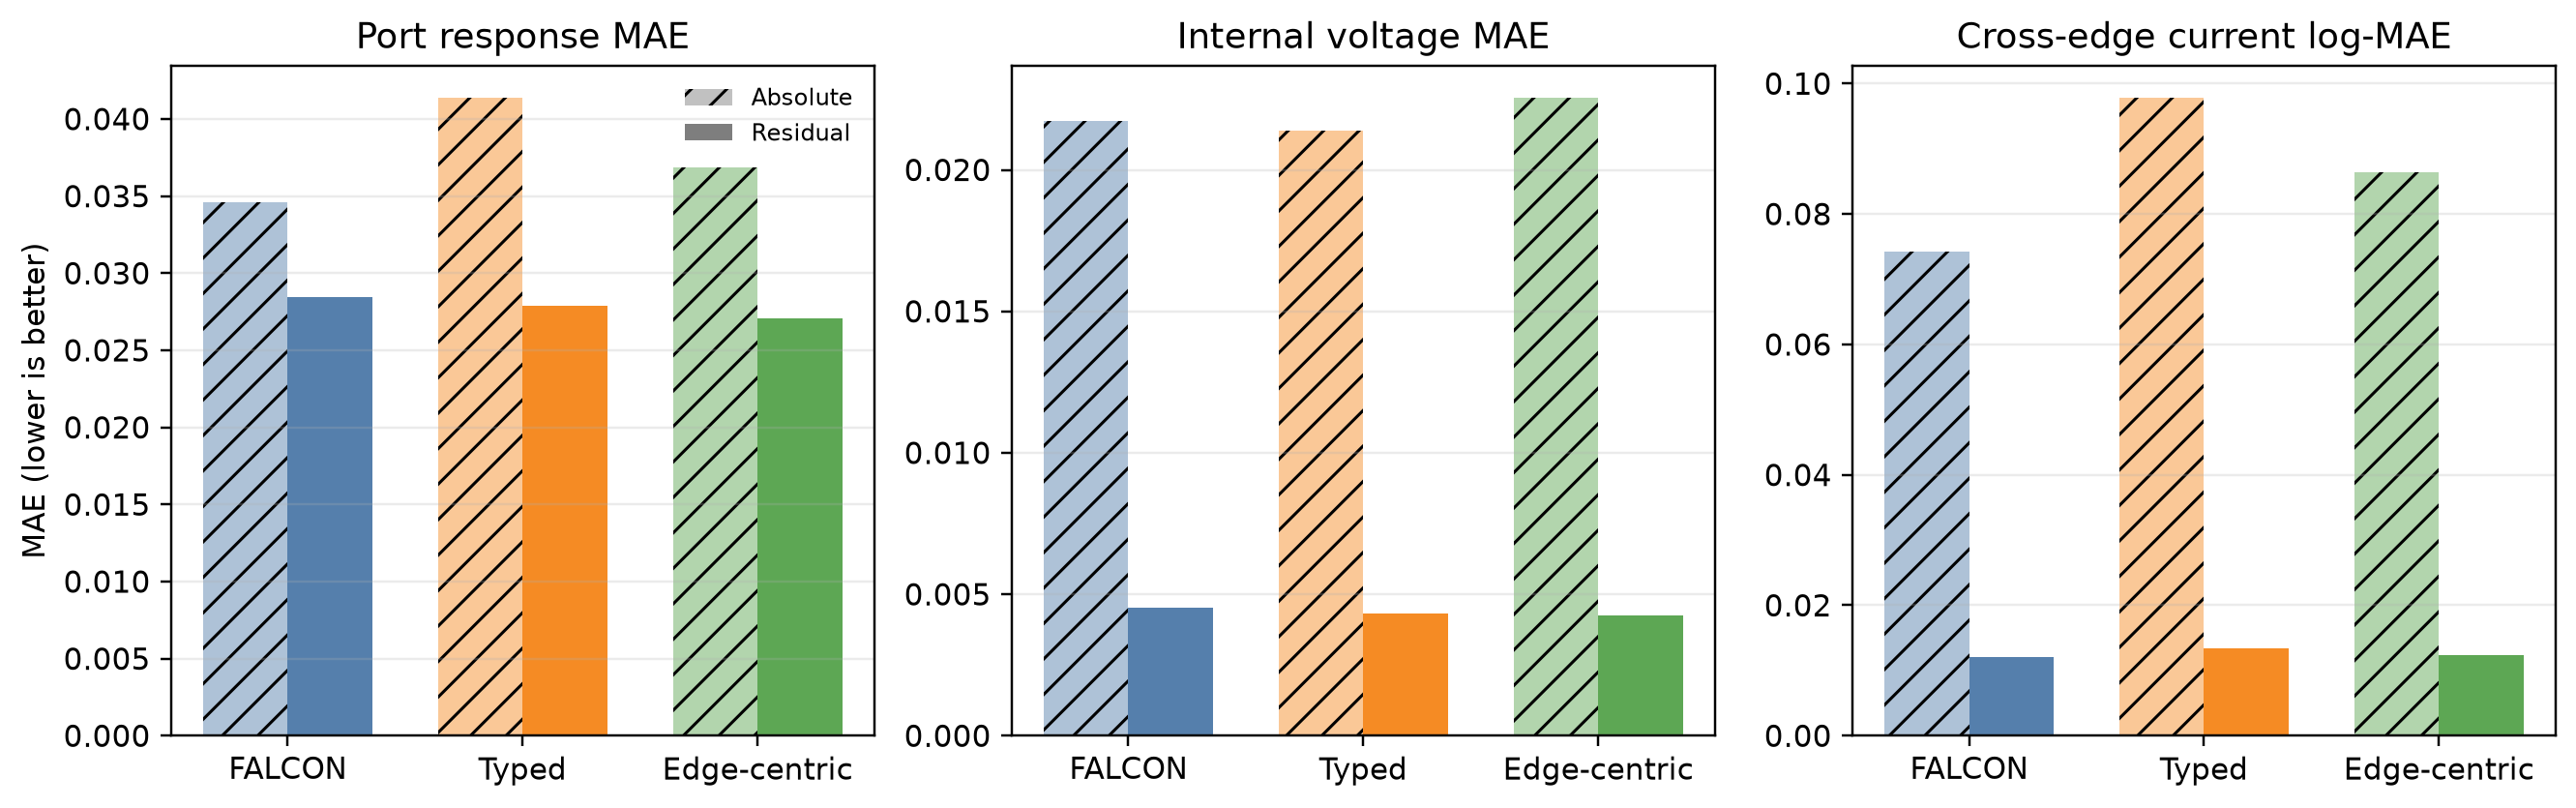
\includegraphics[width=0.98\linewidth]{ablation_absolute_vs_residual.png}
 \caption{绝对目标与局部残差目标消融。残差目标显著降低内部节点误差，并使异构结构在端口和节点任务上出现小幅优势。}
\end{figure}

\begin{figure}[H]
 \centering
 
\includegraphics[width=0.84\linewidth]{residual/test_task_comparison.png}
 \caption{残差任务三模型测试指标。越低越好；边级任务仍由同质基线略占优。}
\end{figure}

\section{失败点与原因定位}
\begin{enumerate}
 \item \textbf{数据层面：}绝对响应主要由 DAB 工况、节点位置和直接边属性决定，局部扰动只是较小分量，掩盖了关系类型的贡献。
 \item \textbf{任务层面：}边电流可由 $C_{ps,ij}$ 和端点电压近似直接决定，当前同质模型已经获得足够线索；同时跨绕组边数随拓扑增加，学习难度上升。
 \item \textbf{架构层面：}edge-centric 模型参数量约为 FALCON 的 2.86 倍，却只得到小幅残差优势，说明当前关系 MLP 尚未实现参数效率优势。边读出缺少显式电流公式解码器和守恒约束。
 \item \textbf{物理约束层面：}教师满足无源性和互易性，但网络只在绝对模式施加端口无源性惩罚；残差本身不是独立无源系统，必须加回标称响应后才能检查。当前残差评估未完成这一重构，因此不能给出预测无源率。
 \item \textbf{定位指标：}残差峰值命中率仅约 12--13\%，且 $8+8$ 拓扑降至约 1--3\%，说明内部局部定位仍是未解决问题。
\end{enumerate}

\section{本实验证明了什么、没有证明什么}
\textbf{已证明：}逐匝图、四类物理边、局部边级扰动、DAB 自然谐波条件、精确矩阵教师和 CUDA 多任务训练链路可以稳定运行；把监督从绝对响应改为同工况局部残差后，显式异构关系对端口响应和内部电压具有可重复的小幅收益。

\textbf{未证明：}异构 GNN 全面优于 FALCON；模型能从真实 DAB 波形反演物理结构；模型能定位真实绝缘缺陷；合成教师能替代 FEM 或实测；当前负载代理量能代表完整负载动态。

\section{下一步建议}
下一步不应继续简单堆网络层数，而应解决边级任务和真实域差距：
\begin{enumerate}
 \item 把位移电流公式作为可微物理解码器：网络预测局部 $\widehat C_{ps,ij}$ 与节点电压，再由 $j\omega C\Delta V$ 计算边电流；
 \item 增加局部 patch 分类/定位辅助头，并采用对扰动区域加权的损失，避免大量弱变化边主导平均误差；
 \item 将 EXP-014 的开关级 DAB/Simulink 输出接入数据契约，加入死区、$C_{\mathrm{oss}}$、接地和测量链路；
 \item 用 Fisher 仅做后验可见性诊断：判断哪些局部更新坐标能由自然 PWM 端口观察，无法区分的边应分组而非强行反演；
 \item 最终采用 COMSOL/FEM 数据预训练，并用少量实测做域适配，检验跨样机泛化。
\end{enumerate}

\section*{复现文件}
主程序为 \texttt{run\_exp18.py}，汇总脚本为 \texttt{summarize\_exp18.py}，快速自检为 \texttt{test\_exp18.py}。两种目标的模型权重、训练历史、逐样本元数据、测试子集和指标分别保存在 \texttt{results/absolute} 与 \texttt{results/residual}。完整正式运行命令和参数可由主程序的命令行帮助获得。

\end{document}
